% Options for packages loaded elsewhere
\PassOptionsToPackage{unicode}{hyperref}
\PassOptionsToPackage{hyphens}{url}
\PassOptionsToPackage{dvipsnames,svgnames,x11names}{xcolor}
%
\documentclass[
  letterpaper,
  DIV=11,
  numbers=noendperiod]{scrreprt}

\usepackage{amsmath,amssymb}
\usepackage{iftex}
\ifPDFTeX
  \usepackage[T1]{fontenc}
  \usepackage[utf8]{inputenc}
  \usepackage{textcomp} % provide euro and other symbols
\else % if luatex or xetex
  \usepackage{unicode-math}
  \defaultfontfeatures{Scale=MatchLowercase}
  \defaultfontfeatures[\rmfamily]{Ligatures=TeX,Scale=1}
\fi
\usepackage{lmodern}
\ifPDFTeX\else  
    % xetex/luatex font selection
\fi
% Use upquote if available, for straight quotes in verbatim environments
\IfFileExists{upquote.sty}{\usepackage{upquote}}{}
\IfFileExists{microtype.sty}{% use microtype if available
  \usepackage[]{microtype}
  \UseMicrotypeSet[protrusion]{basicmath} % disable protrusion for tt fonts
}{}
\makeatletter
\@ifundefined{KOMAClassName}{% if non-KOMA class
  \IfFileExists{parskip.sty}{%
    \usepackage{parskip}
  }{% else
    \setlength{\parindent}{0pt}
    \setlength{\parskip}{6pt plus 2pt minus 1pt}}
}{% if KOMA class
  \KOMAoptions{parskip=half}}
\makeatother
\usepackage{xcolor}
\setlength{\emergencystretch}{3em} % prevent overfull lines
\setcounter{secnumdepth}{5}
% Make \paragraph and \subparagraph free-standing
\ifx\paragraph\undefined\else
  \let\oldparagraph\paragraph
  \renewcommand{\paragraph}[1]{\oldparagraph{#1}\mbox{}}
\fi
\ifx\subparagraph\undefined\else
  \let\oldsubparagraph\subparagraph
  \renewcommand{\subparagraph}[1]{\oldsubparagraph{#1}\mbox{}}
\fi

\usepackage{color}
\usepackage{fancyvrb}
\newcommand{\VerbBar}{|}
\newcommand{\VERB}{\Verb[commandchars=\\\{\}]}
\DefineVerbatimEnvironment{Highlighting}{Verbatim}{commandchars=\\\{\}}
% Add ',fontsize=\small' for more characters per line
\usepackage{framed}
\definecolor{shadecolor}{RGB}{241,243,245}
\newenvironment{Shaded}{\begin{snugshade}}{\end{snugshade}}
\newcommand{\AlertTok}[1]{\textcolor[rgb]{0.68,0.00,0.00}{#1}}
\newcommand{\AnnotationTok}[1]{\textcolor[rgb]{0.37,0.37,0.37}{#1}}
\newcommand{\AttributeTok}[1]{\textcolor[rgb]{0.40,0.45,0.13}{#1}}
\newcommand{\BaseNTok}[1]{\textcolor[rgb]{0.68,0.00,0.00}{#1}}
\newcommand{\BuiltInTok}[1]{\textcolor[rgb]{0.00,0.23,0.31}{#1}}
\newcommand{\CharTok}[1]{\textcolor[rgb]{0.13,0.47,0.30}{#1}}
\newcommand{\CommentTok}[1]{\textcolor[rgb]{0.37,0.37,0.37}{#1}}
\newcommand{\CommentVarTok}[1]{\textcolor[rgb]{0.37,0.37,0.37}{\textit{#1}}}
\newcommand{\ConstantTok}[1]{\textcolor[rgb]{0.56,0.35,0.01}{#1}}
\newcommand{\ControlFlowTok}[1]{\textcolor[rgb]{0.00,0.23,0.31}{#1}}
\newcommand{\DataTypeTok}[1]{\textcolor[rgb]{0.68,0.00,0.00}{#1}}
\newcommand{\DecValTok}[1]{\textcolor[rgb]{0.68,0.00,0.00}{#1}}
\newcommand{\DocumentationTok}[1]{\textcolor[rgb]{0.37,0.37,0.37}{\textit{#1}}}
\newcommand{\ErrorTok}[1]{\textcolor[rgb]{0.68,0.00,0.00}{#1}}
\newcommand{\ExtensionTok}[1]{\textcolor[rgb]{0.00,0.23,0.31}{#1}}
\newcommand{\FloatTok}[1]{\textcolor[rgb]{0.68,0.00,0.00}{#1}}
\newcommand{\FunctionTok}[1]{\textcolor[rgb]{0.28,0.35,0.67}{#1}}
\newcommand{\ImportTok}[1]{\textcolor[rgb]{0.00,0.46,0.62}{#1}}
\newcommand{\InformationTok}[1]{\textcolor[rgb]{0.37,0.37,0.37}{#1}}
\newcommand{\KeywordTok}[1]{\textcolor[rgb]{0.00,0.23,0.31}{#1}}
\newcommand{\NormalTok}[1]{\textcolor[rgb]{0.00,0.23,0.31}{#1}}
\newcommand{\OperatorTok}[1]{\textcolor[rgb]{0.37,0.37,0.37}{#1}}
\newcommand{\OtherTok}[1]{\textcolor[rgb]{0.00,0.23,0.31}{#1}}
\newcommand{\PreprocessorTok}[1]{\textcolor[rgb]{0.68,0.00,0.00}{#1}}
\newcommand{\RegionMarkerTok}[1]{\textcolor[rgb]{0.00,0.23,0.31}{#1}}
\newcommand{\SpecialCharTok}[1]{\textcolor[rgb]{0.37,0.37,0.37}{#1}}
\newcommand{\SpecialStringTok}[1]{\textcolor[rgb]{0.13,0.47,0.30}{#1}}
\newcommand{\StringTok}[1]{\textcolor[rgb]{0.13,0.47,0.30}{#1}}
\newcommand{\VariableTok}[1]{\textcolor[rgb]{0.07,0.07,0.07}{#1}}
\newcommand{\VerbatimStringTok}[1]{\textcolor[rgb]{0.13,0.47,0.30}{#1}}
\newcommand{\WarningTok}[1]{\textcolor[rgb]{0.37,0.37,0.37}{\textit{#1}}}

\providecommand{\tightlist}{%
  \setlength{\itemsep}{0pt}\setlength{\parskip}{0pt}}\usepackage{longtable,booktabs,array}
\usepackage{calc} % for calculating minipage widths
% Correct order of tables after \paragraph or \subparagraph
\usepackage{etoolbox}
\makeatletter
\patchcmd\longtable{\par}{\if@noskipsec\mbox{}\fi\par}{}{}
\makeatother
% Allow footnotes in longtable head/foot
\IfFileExists{footnotehyper.sty}{\usepackage{footnotehyper}}{\usepackage{footnote}}
\makesavenoteenv{longtable}
\usepackage{graphicx}
\makeatletter
\def\maxwidth{\ifdim\Gin@nat@width>\linewidth\linewidth\else\Gin@nat@width\fi}
\def\maxheight{\ifdim\Gin@nat@height>\textheight\textheight\else\Gin@nat@height\fi}
\makeatother
% Scale images if necessary, so that they will not overflow the page
% margins by default, and it is still possible to overwrite the defaults
% using explicit options in \includegraphics[width, height, ...]{}
\setkeys{Gin}{width=\maxwidth,height=\maxheight,keepaspectratio}
% Set default figure placement to htbp
\makeatletter
\def\fps@figure{htbp}
\makeatother

\KOMAoption{captions}{tableheading}
\makeatletter
\@ifpackageloaded{bookmark}{}{\usepackage{bookmark}}
\makeatother
\makeatletter
\@ifpackageloaded{caption}{}{\usepackage{caption}}
\AtBeginDocument{%
\ifdefined\contentsname
  \renewcommand*\contentsname{Table of contents}
\else
  \newcommand\contentsname{Table of contents}
\fi
\ifdefined\listfigurename
  \renewcommand*\listfigurename{List of Figures}
\else
  \newcommand\listfigurename{List of Figures}
\fi
\ifdefined\listtablename
  \renewcommand*\listtablename{List of Tables}
\else
  \newcommand\listtablename{List of Tables}
\fi
\ifdefined\figurename
  \renewcommand*\figurename{Figure}
\else
  \newcommand\figurename{Figure}
\fi
\ifdefined\tablename
  \renewcommand*\tablename{Table}
\else
  \newcommand\tablename{Table}
\fi
}
\@ifpackageloaded{float}{}{\usepackage{float}}
\floatstyle{ruled}
\@ifundefined{c@chapter}{\newfloat{codelisting}{h}{lop}}{\newfloat{codelisting}{h}{lop}[chapter]}
\floatname{codelisting}{Listing}
\newcommand*\listoflistings{\listof{codelisting}{List of Listings}}
\makeatother
\makeatletter
\makeatother
\makeatletter
\@ifpackageloaded{caption}{}{\usepackage{caption}}
\@ifpackageloaded{subcaption}{}{\usepackage{subcaption}}
\makeatother
\ifLuaTeX
  \usepackage{selnolig}  % disable illegal ligatures
\fi
\usepackage{bookmark}

\IfFileExists{xurl.sty}{\usepackage{xurl}}{} % add URL line breaks if available
\urlstyle{same} % disable monospaced font for URLs
\hypersetup{
  pdftitle={Charting Inequality: A Deep Dive into Chicago's Poverty Landscape},
  pdfauthor={Gregory Ho},
  colorlinks=true,
  linkcolor={blue},
  filecolor={Maroon},
  citecolor={Blue},
  urlcolor={Blue},
  pdfcreator={LaTeX via pandoc}}

\title{Charting Inequality: A Deep Dive into Chicago's Poverty
Landscape}
\author{Gregory Ho}
\date{2024-03-05}

\begin{document}
\maketitle

\renewcommand*\contentsname{Table of contents}
{
\hypersetup{linkcolor=}
\setcounter{tocdepth}{2}
\tableofcontents
}
\bookmarksetup{startatroot}

\chapter{Exploring Multidimensional Poverty in the Chicago
Area}\label{exploring-multidimensional-poverty-in-the-chicago-area}

\bookmarksetup{startatroot}

\chapter{Multidimensional Poverty in Cook
County}\label{multidimensional-poverty-in-cook-county}

Within the vibrant urban tapestry of Chicago, characterized by its
architectural prowess and economic vitality, lies a less visible but
critically important dimension of urban life: multidimensional poverty.
This phenomenon extends beyond the traditional income-based assessments,
to encompass a range of deprivations that affect households.

This commentary draws upon the latest empirical data from the ACS 5-Year
Estimates for 2022, employing a methodical approach
(\href{multidimensional_poverty.qmd}{more details here}) to identify and
quantify 15 distinct indicators of deprivation. These indicators span
critical domains such as health, education, employment, housing, and
digital accessibility, thereby offering a comprehensive view of the
multifaceted nature of poverty.

The rationale for adopting a multidimensional perspective on poverty is
grounded in contemporary scholarly discourse, which advocates for a more
nuanced understanding of poverty that reflects the complex realities of
urban deprivation.

\textbf{Consider this - What does poverty really mean in an urban
context?}

It's not just about empty pockets; it's also about being deprived in
many other areas of life, such as quality education, stable jobs, safe
homes, and equitable access in a digitalized world.

\section{The Chicago Deprivation
Canvas}\label{the-chicago-deprivation-canvas}

\textbf{Figure 1: Multidimensional Poverty Indicators in Chicago: A
Factor Analysis}

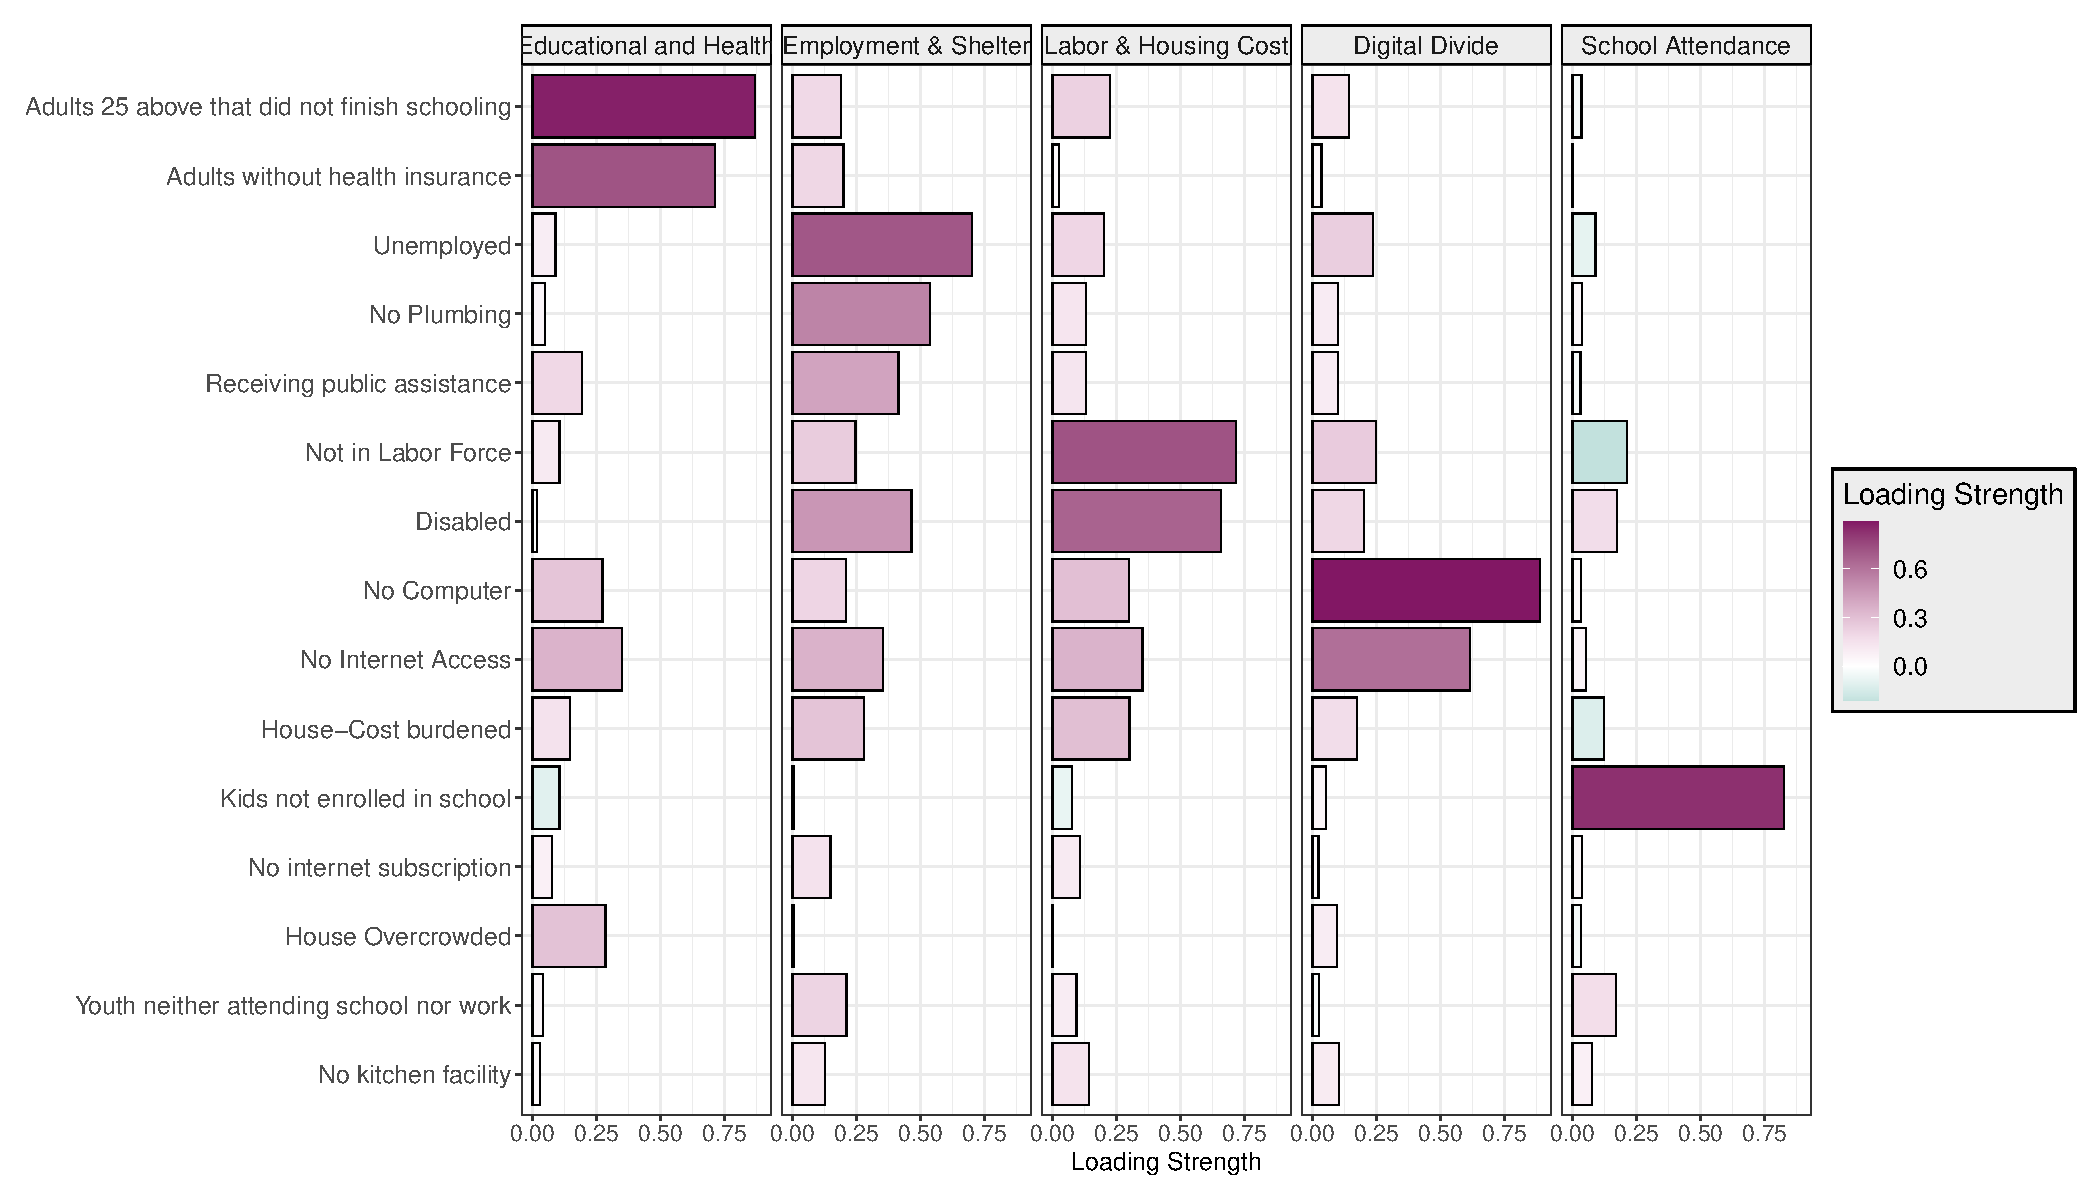
\includegraphics{index_files/figure-pdf/viz1-1.pdf}

Figure 1 presents a factor analysis of various deprivation indicators
within Chicago, offering a statistical representation of the underlying
structures of multidimensional poverty. Factor analysis, a complex
statistical method, is employed here to identify latent variables that
influence the observed data. These latent variables (or factors),
represent broad domains of deprivation that are inferred from the
correlations among the individual indicators. By analyzing these
relationships, the figure visually conveys which aspects of urban life
are most strongly associated with the different facets of poverty.

Each bar on this graph tells a story: a slice of life defined by absence
--- be it in health insurance, a roof over one's head, or a computer in
one's home. These bars stretch out to the extent of their `factor
loading strength,' a numerical representation of how strongly each
indicator resonates with a factor (facet of poverty). Longer bars
signifies a stronger association with a particular facet.

We've dissected the graph into thematic territories, each named for a
facet of deprivation like ``Educational and Health,'' or ``Digital
Divide.'' These are not mere labels but analytical realms --- Multiple
Regression scores that cluster the indicators into meaningful
assemblies. Here, the challenges of poverty don't stand in isolation;
they cluster and often overlap, offering insight into which factors
bundle together in the urban landscape of Chicago.

\bookmarksetup{startatroot}

\chapter{Spatial Distribution of Poverty \& Latent
Factors}\label{spatial-distribution-of-poverty-latent-factors}

\bookmarksetup{startatroot}

\chapter{Figure 2: Spatial Distribution of Poverty \& Latent
Factors}\label{figure-2-spatial-distribution-of-poverty-latent-factors}

The interactive dashboard serves as a tool for dissecting this landscape
of urban poverty. By mapping the contours of poverty's spatial
distribution, this dashboard illuminates the not just ``how much'' but
also the ``where'' of poverty. For example, the pronounced concentration
of \emph{Employment and Shelter} and \emph{Education and Health} within
specific localities underscores the urgent need for targeted policy
interventions. In these identified areas, specific strategies such as
housing initiatives that subsidize renovations, can directly address the
localized nature of these deprivations. Tailoring policies to the unique
characteristics of each neighborhood ensures that resources are
efficiently allocated, directly benefiting those in most need.

Conversely, the more diffused patterns associated with \emph{Labor and
Housing Cost}, \emph{Digital Divide}, and \emph{School Attendance}
suggest systemic issues that pervade beyond individual neighborhoods.
These widespread challenges call for overarching policy frameworks that
address the broader infrastructural and societal deficits. Enhancing
digital infrastructure, for instance, should not only focus on expanding
access but also on ensuring affordability and fostering digital literacy
across the board. Such inclusive strategies are pivotal in bridging the
digital divide, thereby facilitating equitable access to essential
services and opportunities.

\bookmarksetup{startatroot}

\chapter{An analysis of the Digital
Divide}\label{an-analysis-of-the-digital-divide}

In an increasingly digital world, the divide between those with access
to technology and those without is becoming a critical area of concern
for urban development and social equity. This analysis seeks to explore
the relationship between poverty rates and digital accessibility within
Cook County, focusing specifically on households without computers and
those lacking internet access.

\textbf{Figure 3: Poverty rates vs.~Deprivations in Digital Equity}

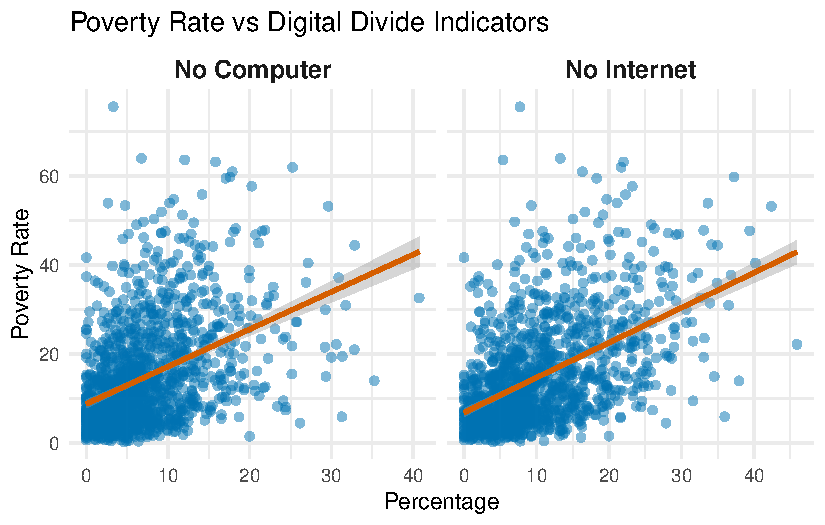
\includegraphics{digital_divide_analysis_files/figure-pdf/viz3_etl-1.pdf}

The visualizations underscore a compelling narrative: areas with higher
poverty rates tend to have a greater percentage of households without
computers and internet access, pointing to a digital divide that mirrors
socioeconomic disparities. This correlation not only highlights the
barriers faced by economically disadvantaged communities in accessing
digital resources but also emphasizes the critical role that digital
accessibility plays in enabling opportunities for education, employment,
and civic participation.

Furthermore from \emph{Figure 2}, given the spatial distribution of this
`digital divide'. This problem is characterized by systemic disparities
that require holistic solutions. Policymakers might take these insights
to re-calibrate resources towards digital literacy programs, affordable
access initiatives, or infrastructure development.

\bookmarksetup{startatroot}

\chapter{Methodology}\label{methodology}

This project is seeks to investigate poverty in Chicago, and the various
deprivations that households face. Data visualizations were produced
using data published in the American Community Survey 5-Year Estimates
as at 2022, compiled by the US Census Bureau.

\section{Instructions to Execute
Code}\label{instructions-to-execute-code}

To reproduce this analysis, an API key from the US Census Bureau is
required. Follow these steps to obtain and use the key:

1.) Request an API key by visiting this
\href{https://api.census.gov/data/key_signup.html}{page} to request a
key

2.) Activate the key using the link sent to your email.

3.) Store the key as an environment variable in your project for secure
access.

Note: Detailed instructions and the code for the analysis are provided
in the accompanying R Markdown document.

\bookmarksetup{startatroot}

\chapter{Multidimensional Poverty}\label{multidimensional-poverty}

The starting point of constructing a Multidimensional Poverty Indicator
would be the generation of a matrix representing tract areas versus
indicators of deprivation.

To generate this matrix, the first step is to identify dimensions of
deprivation that can be constructed using the ACS. These are:

\begin{enumerate}
\def\labelenumi{\arabic{enumi}.}
\item
  Income - percentage receiving public assistance
\item
  Education - percentage of kids not enrolled in school
\item
  Health - percentage of adults without health insurance
\item
  Health - percentage of children with disability status
\item
  Health - percentage of adults with disability status
\item
  Housing - percentage overcrowded: more than 2 occupants per room
\item
  Housing - percentage cost-burdened
\item
  Living Conditions - percentage without plumbing facilities
\item
  Living Conditions - percentage without kitchen facilities
\item
  Digitalization - percentage without computer
\item
  Digitalization - percentage without internet access
\item
  Digitalization - percentage internet access without subscription
\item
  Employment - percent unemployed
\item
  Employment - percent not in labor force
\end{enumerate}

\bookmarksetup{startatroot}

\chapter{Deprivation Cutoffs}\label{deprivation-cutoffs}

Typically, deprivation cutoffs are thresholds used to determine whether
a household is considered deprived in a particular dimension. These
cutoffs are crucial in generating a raw deprivation matrix, as they help
to classify the population into different categories based on their
level of deprivation.

In our case, we deviate from the standard practice by setting the
deprivation cutoffs at 0\%. This means that we consider any level of
deprivation within a household as significant enough to count towards
the overall deprivation score for a census tract. By employing this
approach, we are able to capture the full spectrum of deprivation
levels, from the most mild to the most severe.

\begin{Shaded}
\begin{Highlighting}[]
\NormalTok{deprivation\_percentages }\OtherTok{\textless{}{-}}\NormalTok{ chicago\_data\_deprivation }\SpecialCharTok{\%\textgreater{}\%}
  \FunctionTok{mutate}\NormalTok{(}
    \CommentTok{\# Income}
    \CommentTok{\#Pct\_Below\_Poverty = (total\_below\_povertyE / poverty\_totalE) * 100,}
    \AttributeTok{Pct\_Receiving\_PA =}\NormalTok{ (total\_recieve\_paE }\SpecialCharTok{/}\NormalTok{ recieve\_pa\_totalE) }\SpecialCharTok{*} \DecValTok{100}\NormalTok{,}
    
    \CommentTok{\# Education}
    \AttributeTok{Pct\_Kids\_Not\_In\_School =}\NormalTok{ (kids\_Not\_In\_SchoolE }\SpecialCharTok{/}\NormalTok{ kids\_totalE) }\SpecialCharTok{*} \DecValTok{100}\NormalTok{,}
    \AttributeTok{Pct\_Youth\_Not\_In\_School\_Not\_Working =}\NormalTok{ ((youth\_male\_xschool\_unemployedE }\SpecialCharTok{+}\NormalTok{ youth\_male\_xschool\_xlfE }\SpecialCharTok{+} 
\NormalTok{                                            youth\_female\_xschool\_unemployedE }\SpecialCharTok{+}\NormalTok{ youth\_female\_xschool\_xlfE) }\SpecialCharTok{/}\NormalTok{ youth\_totalE) }\SpecialCharTok{*} \DecValTok{100}\NormalTok{,}
    \AttributeTok{Pct\_Adults\_No\_HighSchool =}\NormalTok{ ((abv25\_no\_schoolE }\SpecialCharTok{+}\NormalTok{ abv25\_nurseryE }\SpecialCharTok{+}\NormalTok{ abv25\_kindergartenE }\SpecialCharTok{+}\NormalTok{ abv25\_g1E }\SpecialCharTok{+} 
\NormalTok{                                 abv25\_g2E }\SpecialCharTok{+}\NormalTok{ abv25\_g3E }\SpecialCharTok{+}\NormalTok{ abv25\_g4E }\SpecialCharTok{+}\NormalTok{ abv25\_g5E }\SpecialCharTok{+}\NormalTok{ abv25\_g6E }\SpecialCharTok{+} 
\NormalTok{                                 abv25\_g7E }\SpecialCharTok{+}\NormalTok{ abv25\_g8E }\SpecialCharTok{+}\NormalTok{ abv25\_g9E }\SpecialCharTok{+}\NormalTok{ abv25\_g10E }\SpecialCharTok{+}\NormalTok{ abv25\_g11E }\SpecialCharTok{+} 
\NormalTok{                                 abv25\_g12E) }\SpecialCharTok{/}\NormalTok{ total\_abv25E) }\SpecialCharTok{*} \DecValTok{100}\NormalTok{,}
    
    \CommentTok{\# Health}
    \AttributeTok{Pct\_Disabled =}\NormalTok{ ((dis\_male\_4E }\SpecialCharTok{+}\NormalTok{ dis\_male\_5\_17E }\SpecialCharTok{+}\NormalTok{ dis\_male\_18\_34E }\SpecialCharTok{+}\NormalTok{ dis\_male\_35\_64E }\SpecialCharTok{+} 
\NormalTok{                     dis\_male\_65\_74E }\SpecialCharTok{+}\NormalTok{ dis\_male\_75E }\SpecialCharTok{+}\NormalTok{ dis\_female\_4E }\SpecialCharTok{+}\NormalTok{ dis\_female\_5\_17E }\SpecialCharTok{+} 
\NormalTok{                     dis\_female\_18\_34E }\SpecialCharTok{+}\NormalTok{ dis\_female\_35\_64E }\SpecialCharTok{+}\NormalTok{ dis\_female\_65\_74E }\SpecialCharTok{+} 
\NormalTok{                     dis\_female\_75E) }\SpecialCharTok{/}\NormalTok{ dis\_totalE) }\SpecialCharTok{*} \DecValTok{100}\NormalTok{,}
    \AttributeTok{Pct\_No\_Insurance =}\NormalTok{ ((no\_ins\_dis\_18E }\SpecialCharTok{+}\NormalTok{ no\_ins\_xdis\_18E }\SpecialCharTok{+}\NormalTok{ no\_ins\_dis\_19\_64E }\SpecialCharTok{+} 
\NormalTok{                         no\_ins\_xdis\_19\_64E }\SpecialCharTok{+}\NormalTok{ no\_ins\_dis\_65E }\SpecialCharTok{+}\NormalTok{ no\_ins\_xdis\_65E) }\SpecialCharTok{/}\NormalTok{ ins\_totalE) }\SpecialCharTok{*} \DecValTok{100}\NormalTok{,}
    
    \CommentTok{\# Housing}
    \AttributeTok{Pct\_Overcrowded\_Housing =}\NormalTok{ ((Overcrowded\_Housing\_ownE }\SpecialCharTok{+}\NormalTok{ Overcrowded\_Housing\_rentE) }\SpecialCharTok{/}\NormalTok{ housing\_totalE) }\SpecialCharTok{*} \DecValTok{100}\NormalTok{,}
    \AttributeTok{Pct\_Cost\_Burdened\_Housing =}\NormalTok{ ((cost\_burdened\_housing\_30\_35E }\SpecialCharTok{+}\NormalTok{ cost\_burdened\_housing\_35\_40E }\SpecialCharTok{+} 
\NormalTok{                                  cost\_burdened\_housing\_40\_50E }\SpecialCharTok{+}\NormalTok{ cost\_burdened\_housing\_50\_aboveE) }\SpecialCharTok{/} 
\NormalTok{                                  cost\_burdened\_housing\_totalE) }\SpecialCharTok{*} \DecValTok{100}\NormalTok{,}
    
    \CommentTok{\# Living Conditions}
    \AttributeTok{Pct\_No\_Plumbing =}\NormalTok{ (no\_plumbingE }\SpecialCharTok{/}\NormalTok{ total\_housing\_plumbingE) }\SpecialCharTok{*} \DecValTok{100}\NormalTok{,}
    \AttributeTok{Pct\_No\_Kitchen =}\NormalTok{ ((no\_kitchen\_ownE }\SpecialCharTok{+}\NormalTok{ no\_kitchen\_rentE) }\SpecialCharTok{/}\NormalTok{ total\_housing\_kitchenE) }\SpecialCharTok{*} \DecValTok{100}\NormalTok{,}
    
    \CommentTok{\# Digital Divide}
    \AttributeTok{Pct\_No\_Computer =}\NormalTok{ (no\_computerE }\SpecialCharTok{/}\NormalTok{ total\_householdsE) }\SpecialCharTok{*} \DecValTok{100}\NormalTok{,}
    \AttributeTok{Pct\_No\_Internet =}\NormalTok{ (no\_internetE }\SpecialCharTok{/}\NormalTok{ total\_householdsE) }\SpecialCharTok{*} \DecValTok{100}\NormalTok{,}
    \AttributeTok{Pct\_Internet\_No\_Subscription =}\NormalTok{ (internet\_no\_subscriptionE }\SpecialCharTok{/}\NormalTok{ total\_householdsE) }\SpecialCharTok{*} \DecValTok{100}\NormalTok{,}
    
    \CommentTok{\# Employment}
    \AttributeTok{Pct\_Unemployed =}\NormalTok{ (unemployedE }\SpecialCharTok{/}\NormalTok{ workforce\_totalE) }\SpecialCharTok{*} \DecValTok{100}\NormalTok{,}
    \AttributeTok{Pct\_Not\_In\_Labor\_Force =}\NormalTok{ (not\_in\_labor\_forceE }\SpecialCharTok{/}\NormalTok{ pop\_employment\_totalE) }\SpecialCharTok{*} \DecValTok{100}
\NormalTok{  ) }\SpecialCharTok{\%\textgreater{}\%}
  \FunctionTok{select}\NormalTok{(GEOID, }\FunctionTok{starts\_with}\NormalTok{(}\StringTok{"Pct\_"}\NormalTok{))  }\CommentTok{\# Keep only GEOID and calculated percentages}
\end{Highlighting}
\end{Shaded}

\bookmarksetup{startatroot}

\chapter{Exploratory Factor Analysis}\label{exploratory-factor-analysis}

\begin{Shaded}
\begin{Highlighting}[]
\FunctionTok{library}\NormalTok{(psych)}
\end{Highlighting}
\end{Shaded}

\begin{verbatim}
Warning: package 'psych' was built under R version 4.2.3
\end{verbatim}

\begin{verbatim}

Attaching package: 'psych'
\end{verbatim}

\begin{verbatim}
The following objects are masked from 'package:ggplot2':

    %+%, alpha
\end{verbatim}

\begin{Shaded}
\begin{Highlighting}[]
\CommentTok{\# Exclude non{-}numeric variables if any}
\NormalTok{deprivation\_factors }\OtherTok{\textless{}{-}}\NormalTok{ deprivation\_percentages }\SpecialCharTok{\%\textgreater{}\%} 
  \FunctionTok{select}\NormalTok{(}\SpecialCharTok{{-}}\NormalTok{GEOID) }\SpecialCharTok{\%\textgreater{}\%}  \CommentTok{\# Exclude GEOID or any other non{-}numeric variables}
  \FunctionTok{select\_if}\NormalTok{(is.numeric)  }\CommentTok{\# Select only numeric columns}

\CommentTok{\# Check for NA values and decide on handling strategy}
\FunctionTok{summary}\NormalTok{(deprivation\_factors)}
\end{Highlighting}
\end{Shaded}

\begin{verbatim}
 Pct_Receiving_PA Pct_Kids_Not_In_School Pct_Youth_Not_In_School_Not_Working
 Min.   : 0.000   Min.   :11.93          Min.   :  0.000                    
 1st Qu.: 1.048   1st Qu.:71.68          1st Qu.:  0.000                    
 Median : 2.371   Median :75.69          Median :  0.000                    
 Mean   : 3.301   Mean   :75.33          Mean   :  2.632                    
 3rd Qu.: 4.700   3rd Qu.:80.09          3rd Qu.:  0.000                    
 Max.   :21.964   Max.   :97.30          Max.   :100.000                    
 NA's   :4        NA's   :4              NA's   :25                         
 Pct_Adults_No_HighSchool  Pct_Disabled     Pct_No_Insurance
 Min.   : 0.000           Min.   : 0.3284   Min.   : 0.000  
 1st Qu.: 4.378           1st Qu.: 7.4678   1st Qu.: 3.944  
 Median : 9.984           Median :10.1953   Median : 7.590  
 Mean   :12.407           Mean   :11.4048   Mean   : 8.976  
 3rd Qu.:17.967           3rd Qu.:14.3950   3rd Qu.:12.783  
 Max.   :52.635           Max.   :37.9172   Max.   :41.686  
 NA's   :4                NA's   :4         NA's   :4       
 Pct_Overcrowded_Housing Pct_Cost_Burdened_Housing Pct_No_Plumbing  
 Min.   :0.0000          Min.   :  0.00            Min.   : 0.0000  
 1st Qu.:0.0000          1st Qu.: 34.68            1st Qu.: 0.0000  
 Median :0.0000          Median : 45.13            Median : 0.6113  
 Mean   :0.3091          Mean   : 45.73            Mean   : 2.1149  
 3rd Qu.:0.0000          3rd Qu.: 56.67            3rd Qu.: 2.5272  
 Max.   :7.5419          Max.   :100.00            Max.   :39.0738  
 NA's   :4               NA's   :7                 NA's   :4        
 Pct_No_Kitchen    Pct_No_Computer  Pct_No_Internet 
 Min.   : 0.0000   Min.   : 0.000   Min.   : 0.000  
 1st Qu.: 0.0000   1st Qu.: 2.820   1st Qu.: 4.194  
 Median : 0.0000   Median : 5.722   Median : 8.173  
 Mean   : 0.7670   Mean   : 7.104   Mean   :10.065  
 3rd Qu.: 0.8996   3rd Qu.: 9.988   3rd Qu.:14.204  
 Max.   :13.8008   Max.   :40.765   Max.   :45.918  
 NA's   :4         NA's   :4        NA's   :4       
 Pct_Internet_No_Subscription Pct_Unemployed   Pct_Not_In_Labor_Force
 Min.   : 0.0000              Min.   : 0.000   Min.   : 5.971        
 1st Qu.: 0.6063              1st Qu.: 3.571   1st Qu.:28.549        
 Median : 1.7697              Median : 6.085   Median :34.457        
 Mean   : 2.7185              Mean   : 8.300   Mean   :34.365        
 3rd Qu.: 3.8625              3rd Qu.:10.737   3rd Qu.:40.961        
 Max.   :21.9839              Max.   :47.742   Max.   :94.788        
 NA's   :4                    NA's   :4        NA's   :4             
\end{verbatim}

\begin{Shaded}
\begin{Highlighting}[]
\NormalTok{fa\_result }\OtherTok{\textless{}{-}} \FunctionTok{fa}\NormalTok{(deprivation\_factors, }\AttributeTok{nfactors =} \DecValTok{5}\NormalTok{, }\AttributeTok{rotate =} \StringTok{"varimax"}\NormalTok{, }\AttributeTok{fm =} \StringTok{"minres"}\NormalTok{)}

\CommentTok{\# Print the factor analysis results}
\FunctionTok{print}\NormalTok{(fa\_result)}
\end{Highlighting}
\end{Shaded}

\begin{verbatim}
Factor Analysis using method =  minres
Call: fa(r = deprivation_factors, nfactors = 5, rotate = "varimax", 
    fm = "minres")
Standardized loadings (pattern matrix) based upon correlation matrix
                                      MR2   MR4   MR1   MR5   MR3    h2     u2
Pct_Receiving_PA                     0.19  0.41  0.13  0.10 -0.03 0.237 0.7629
Pct_Kids_Not_In_School              -0.11 -0.01 -0.08  0.05  0.83 0.702 0.2979
Pct_Youth_Not_In_School_Not_Working  0.04  0.21  0.09 -0.03  0.17 0.084 0.9157
Pct_Adults_No_HighSchool             0.87  0.19  0.23  0.14 -0.03 0.862 0.1381
Pct_Disabled                        -0.02  0.46  0.66  0.20  0.17 0.720 0.2796
Pct_No_Insurance                     0.71  0.20  0.03  0.03  0.00 0.551 0.4493
Pct_Overcrowded_Housing              0.29  0.01  0.00  0.09 -0.03 0.092 0.9084
Pct_Cost_Burdened_Housing            0.15  0.28  0.30  0.17 -0.12 0.236 0.7643
Pct_No_Plumbing                      0.05  0.54  0.13  0.10  0.04 0.320 0.6802
Pct_No_Kitchen                       0.03  0.13  0.14  0.10  0.08 0.053 0.9465
Pct_No_Computer                      0.27  0.21  0.30  0.89  0.03 0.997 0.0025
Pct_No_Internet                      0.35  0.35  0.35  0.61  0.05 0.752 0.2477
Pct_Internet_No_Subscription         0.08  0.15  0.11  0.02  0.04 0.041 0.9587
Pct_Unemployed                       0.09  0.70  0.20  0.24 -0.09 0.605 0.3947
Pct_Not_In_Labor_Force               0.11  0.25  0.72  0.25 -0.21 0.690 0.3098
                                    com
Pct_Receiving_PA                    1.8
Pct_Kids_Not_In_School              1.1
Pct_Youth_Not_In_School_Not_Working 2.5
Pct_Adults_No_HighSchool            1.3
Pct_Disabled                        2.2
Pct_No_Insurance                    1.2
Pct_Overcrowded_Housing             1.2
Pct_Cost_Burdened_Housing           3.5
Pct_No_Plumbing                     1.2
Pct_No_Kitchen                      3.5
Pct_No_Computer                     1.6
Pct_No_Internet                     3.0
Pct_Internet_No_Subscription        2.6
Pct_Unemployed                      1.5
Pct_Not_In_Labor_Force              1.8

                       MR2  MR4  MR1  MR5  MR3
SS loadings           1.64 1.64 1.42 1.42 0.82
Proportion Var        0.11 0.11 0.09 0.09 0.05
Cumulative Var        0.11 0.22 0.31 0.41 0.46
Proportion Explained  0.24 0.24 0.20 0.20 0.12
Cumulative Proportion 0.24 0.47 0.68 0.88 1.00

Mean item complexity =  2
Test of the hypothesis that 5 factors are sufficient.

df null model =  105  with the objective function =  4.6 with Chi Square =  6101.43
df of  the model are 40  and the objective function was  0.09 

The root mean square of the residuals (RMSR) is  0.02 
The df corrected root mean square of the residuals is  0.03 

The harmonic n.obs is  1325 with the empirical chi square  85.88  with prob <  3.4e-05 
The total n.obs was  1332  with Likelihood Chi Square =  115.98  with prob <  2.5e-09 

Tucker Lewis Index of factoring reliability =  0.967
RMSEA index =  0.038  and the 90 % confidence intervals are  0.03 0.046
BIC =  -171.8
Fit based upon off diagonal values = 1
Measures of factor score adequacy             
                                                   MR2  MR4  MR1  MR5  MR3
Correlation of (regression) scores with factors   0.92 0.80 0.82 0.98 0.85
Multiple R square of scores with factors          0.85 0.65 0.66 0.96 0.72
Minimum correlation of possible factor scores     0.71 0.30 0.33 0.93 0.44
\end{verbatim}

\begin{Shaded}
\begin{Highlighting}[]
\FunctionTok{print}\NormalTok{(fa\_result}\SpecialCharTok{$}\NormalTok{values)}
\end{Highlighting}
\end{Shaded}

\begin{verbatim}
 [1]  4.085341333  1.108575875  0.826211308  0.597304147  0.327840052
 [6]  0.144707267  0.082097939  0.053076216  0.025620213  0.021642830
[11] -0.009223714 -0.043425297 -0.052486179 -0.070706753 -0.153102481
\end{verbatim}

\begin{Shaded}
\begin{Highlighting}[]
\CommentTok{\# Plot the factor loadings for a visual representation}
\FunctionTok{fa.diagram}\NormalTok{(fa\_result)}
\end{Highlighting}
\end{Shaded}

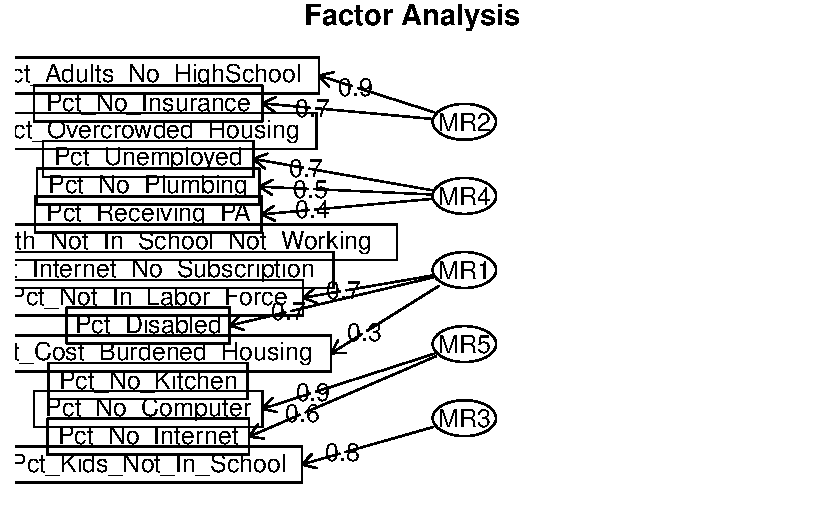
\includegraphics{multidimensional_poverty_files/figure-pdf/factor-1.pdf}

\begin{Shaded}
\begin{Highlighting}[]
\CommentTok{\# Parallel}
\FunctionTok{fa.parallel}\NormalTok{(deprivation\_factors, }\AttributeTok{fm =} \StringTok{"minres"}\NormalTok{, }\AttributeTok{fa =} \StringTok{"fa"}\NormalTok{)}
\end{Highlighting}
\end{Shaded}

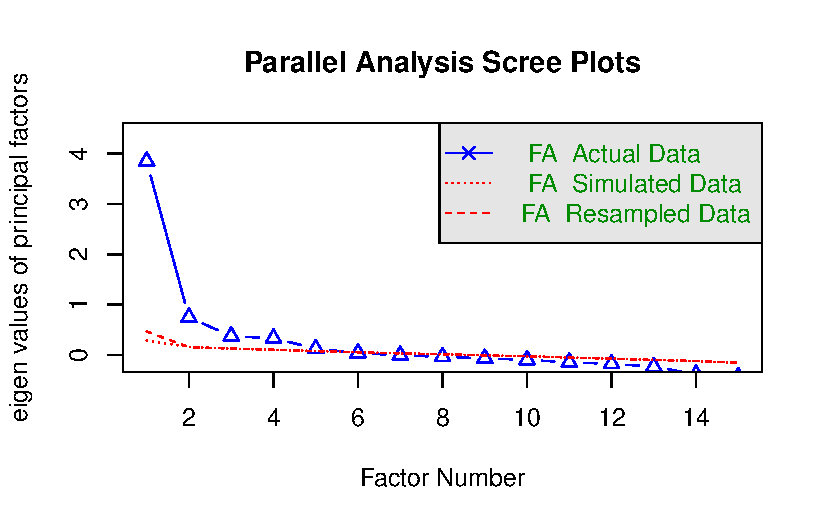
\includegraphics{multidimensional_poverty_files/figure-pdf/factor-2.pdf}

\begin{verbatim}
Parallel analysis suggests that the number of factors =  5  and the number of components =  NA 
\end{verbatim}

\begin{Shaded}
\begin{Highlighting}[]
\CommentTok{\# Examine factor loadings}
\NormalTok{loadings }\OtherTok{\textless{}{-}}\NormalTok{ fa\_result}\SpecialCharTok{$}\NormalTok{loadings}

\CommentTok{\# Print factor loadings for interpretation}
\FunctionTok{print}\NormalTok{(loadings)}
\end{Highlighting}
\end{Shaded}

\begin{verbatim}

Loadings:
                                    MR2    MR4    MR1    MR5    MR3   
Pct_Receiving_PA                     0.193  0.414  0.131              
Pct_Kids_Not_In_School              -0.106                       0.826
Pct_Youth_Not_In_School_Not_Working         0.212                0.168
Pct_Adults_No_HighSchool             0.868  0.189  0.225  0.143       
Pct_Disabled                                0.465  0.659  0.200  0.173
Pct_No_Insurance                     0.714  0.199                     
Pct_Overcrowded_Housing              0.285                            
Pct_Cost_Burdened_Housing            0.147  0.280  0.301  0.173 -0.123
Pct_No_Plumbing                             0.538  0.130  0.100       
Pct_No_Kitchen                              0.127  0.143  0.102       
Pct_No_Computer                      0.274  0.208  0.300  0.888       
Pct_No_Internet                      0.350  0.354  0.352  0.615       
Pct_Internet_No_Subscription                0.149  0.107              
Pct_Unemployed                              0.702  0.202  0.236       
Pct_Not_In_Labor_Force               0.106  0.246  0.716  0.248 -0.211

                 MR2   MR4   MR1   MR5   MR3
SS loadings    1.643 1.636 1.423 1.418 0.824
Proportion Var 0.110 0.109 0.095 0.095 0.055
Cumulative Var 0.110 0.219 0.313 0.408 0.463
\end{verbatim}

\begin{Shaded}
\begin{Highlighting}[]
\FunctionTok{library}\NormalTok{(reshape2)}
\end{Highlighting}
\end{Shaded}

\begin{verbatim}
Warning: package 'reshape2' was built under R version 4.2.3
\end{verbatim}

\begin{verbatim}

Attaching package: 'reshape2'
\end{verbatim}

\begin{verbatim}
The following object is masked from 'package:tidyr':

    smiths
\end{verbatim}

\begin{Shaded}
\begin{Highlighting}[]
\FunctionTok{library}\NormalTok{(ggplot2)}

\CommentTok{\# Extract loadings matrix}
\NormalTok{loadings\_matrix }\OtherTok{\textless{}{-}}\NormalTok{ fa\_result}\SpecialCharTok{$}\NormalTok{loadings}

\CommentTok{\# Assuming the last 3 rows are SS loadings, prop. var., and cum. var., remove them}
\NormalTok{loadings\_matrix\_clean }\OtherTok{\textless{}{-}}\NormalTok{ loadings\_matrix[}\DecValTok{1}\SpecialCharTok{:}\NormalTok{(}\FunctionTok{nrow}\NormalTok{(loadings\_matrix)), ]}

\CommentTok{\# Convert clean loadings matrix to a dataframe}
\NormalTok{loadings\_df }\OtherTok{\textless{}{-}} \FunctionTok{as.data.frame}\NormalTok{(loadings\_matrix\_clean)}

\CommentTok{\# Add row names as a new column for variable names}
\NormalTok{loadings\_df}\SpecialCharTok{$}\NormalTok{Variable }\OtherTok{\textless{}{-}} \FunctionTok{rownames}\NormalTok{(loadings\_df)}

\CommentTok{\# Define the order}
\NormalTok{Ord }\OtherTok{\textless{}{-}} \FunctionTok{rev}\NormalTok{(}\FunctionTok{c}\NormalTok{(}\StringTok{"Pct\_Adults\_No\_HighSchool"}\NormalTok{,}
         \StringTok{"Pct\_No\_Insurance"}\NormalTok{,}
         \StringTok{"Pct\_Unemployed"}\NormalTok{,}
         \StringTok{"Pct\_No\_Plumbing"}\NormalTok{,}
         \StringTok{"Pct\_Receiving\_PA"}\NormalTok{,}
         \StringTok{"Pct\_Not\_In\_Labor\_Force"}\NormalTok{,}
         \StringTok{"Pct\_Disabled"}\NormalTok{,}
         \StringTok{"Pct\_No\_Computer"}\NormalTok{,}
         \StringTok{"Pct\_No\_Internet"}\NormalTok{,}
         \StringTok{"Pct\_Cost\_Burdened\_Housing"}\NormalTok{,}
         \StringTok{"Pct\_Kids\_Not\_In\_School"}\NormalTok{,}
         \StringTok{"Pct\_Internet\_No\_Subscription"}\NormalTok{,}
         \StringTok{"Pct\_Overcrowded\_Housing"}\NormalTok{,}
         \StringTok{"Pct\_Youth\_Not\_In\_School\_Not\_Working"}\NormalTok{,}
         \StringTok{"Pct\_No\_Kitchen"}
\NormalTok{         ))}

\CommentTok{\# Set the factor levels based on the order}
\NormalTok{loadings\_df}\SpecialCharTok{$}\NormalTok{Variable }\OtherTok{\textless{}{-}} \FunctionTok{factor}\NormalTok{(loadings\_df}\SpecialCharTok{$}\NormalTok{Variable, }\AttributeTok{levels =}\NormalTok{ Ord)}

\CommentTok{\# Optionally rename the factor columns}
\CommentTok{\# This depends on how many factors you have}
\FunctionTok{colnames}\NormalTok{(loadings\_df)[}\DecValTok{1}\SpecialCharTok{:}\FunctionTok{ncol}\NormalTok{(loadings\_df)}\SpecialCharTok{{-}}\DecValTok{1}\NormalTok{] }\OtherTok{\textless{}{-}} \FunctionTok{c}\NormalTok{(}\StringTok{"Educational and Health"}\NormalTok{,}
                                                  \StringTok{"Employment \& Home Condition"}\NormalTok{,}
                                                  \StringTok{"Labor \& Housing Cost"}\NormalTok{,}
                                                  \StringTok{"Digital Divide"}\NormalTok{,}
                                                  \StringTok{"School Attendance"}\NormalTok{)}

\CommentTok{\# Melt the dataframe}
\NormalTok{loadings\_long }\OtherTok{\textless{}{-}} \FunctionTok{melt}\NormalTok{(loadings\_df, }\AttributeTok{id.vars =} \StringTok{"Variable"}\NormalTok{, }\AttributeTok{variable.name =} \StringTok{"Factor"}\NormalTok{, }\AttributeTok{value.name =} \StringTok{"Loading"}\NormalTok{)}

\CommentTok{\# Now, rename the levels of the Variable factor}
\NormalTok{loadings\_long}\SpecialCharTok{$}\NormalTok{Variable }\OtherTok{\textless{}{-}} \FunctionTok{factor}\NormalTok{(loadings\_long}\SpecialCharTok{$}\NormalTok{Variable, }\AttributeTok{levels =}\NormalTok{ Ord,}
                                 \AttributeTok{labels =} \FunctionTok{rev}\NormalTok{(}\FunctionTok{c}\NormalTok{(}\StringTok{\textquotesingle{}Adults 25 above that did not finish schooling\textquotesingle{}}\NormalTok{,}
                                            \StringTok{\textquotesingle{}Adults without health insurance\textquotesingle{}}\NormalTok{,}
                                            \StringTok{\textquotesingle{}Unemployed\textquotesingle{}}\NormalTok{,}
                                            \StringTok{\textquotesingle{}No Plumbing\textquotesingle{}}\NormalTok{,}
                                            \StringTok{\textquotesingle{}Receiving public assistance\textquotesingle{}}\NormalTok{,}
                                            \StringTok{\textquotesingle{}Not in Labor Force\textquotesingle{}}\NormalTok{,}
                                            \StringTok{\textquotesingle{}Disabled\textquotesingle{}}\NormalTok{,}
                                            \StringTok{\textquotesingle{}No Computer\textquotesingle{}}\NormalTok{,}
                                            \StringTok{\textquotesingle{}No Internet Access\textquotesingle{}}\NormalTok{,}
                                            \StringTok{\textquotesingle{}House{-}Cost burdened\textquotesingle{}}\NormalTok{,}
                                            \StringTok{\textquotesingle{}Kids not enrolled in school\textquotesingle{}}\NormalTok{,}
                                            \StringTok{\textquotesingle{}No internet subscription\textquotesingle{}}\NormalTok{,}
                                            \StringTok{\textquotesingle{}House Overcrowded\textquotesingle{}}\NormalTok{,}
                                            \StringTok{\textquotesingle{}Youth neither attending school nor work\textquotesingle{}}\NormalTok{,}
                                            \StringTok{\textquotesingle{}No kitchen facility\textquotesingle{}}\NormalTok{)))}

\CommentTok{\# Plot}
\FunctionTok{library}\NormalTok{(}\StringTok{"colorspace"}\NormalTok{)}
\end{Highlighting}
\end{Shaded}

\begin{verbatim}
Warning: package 'colorspace' was built under R version 4.2.3
\end{verbatim}

\begin{Shaded}
\begin{Highlighting}[]
\FunctionTok{ggplot}\NormalTok{(loadings\_long, }\FunctionTok{aes}\NormalTok{(Variable, }\FunctionTok{abs}\NormalTok{(Loading), }\AttributeTok{fill=}\NormalTok{Loading)) }\SpecialCharTok{+} 
  \FunctionTok{facet\_wrap}\NormalTok{(}\SpecialCharTok{\textasciitilde{}}\NormalTok{ Factor, }\AttributeTok{nrow=}\DecValTok{1}\NormalTok{) }\SpecialCharTok{+} 
  \FunctionTok{geom\_bar}\NormalTok{(}\AttributeTok{stat=}\StringTok{"identity"}\NormalTok{, }\AttributeTok{color=}\StringTok{"grey"}\NormalTok{) }\SpecialCharTok{+} 
  \FunctionTok{coord\_flip}\NormalTok{() }\SpecialCharTok{+} 
  \FunctionTok{scale\_fill\_continuous\_diverging}\NormalTok{(}\AttributeTok{palette =} \StringTok{"Cyan{-}Mage"}\NormalTok{, }\AttributeTok{l1 =} \DecValTok{30}\NormalTok{, }\AttributeTok{l2 =} \DecValTok{100}\NormalTok{, }\AttributeTok{p1 =}\NormalTok{ .}\DecValTok{9}\NormalTok{, }\AttributeTok{p2 =} \FloatTok{1.2}\NormalTok{) }\SpecialCharTok{+}
  \FunctionTok{labs}\NormalTok{(}\AttributeTok{x=} \StringTok{"Dimension of Deprivation"}\NormalTok{, }\AttributeTok{y =} \StringTok{"Loading Strength"}\NormalTok{, }\AttributeTok{fill =} \StringTok{"Loading Strength"}\NormalTok{) }\SpecialCharTok{+}
  \FunctionTok{theme\_bw}\NormalTok{(}\AttributeTok{base\_size=}\DecValTok{10}\NormalTok{) }\SpecialCharTok{+}
  \FunctionTok{theme}\NormalTok{(}
    \AttributeTok{strip.text =} \FunctionTok{element\_text}\NormalTok{(}\AttributeTok{size =} \DecValTok{12}\NormalTok{),}
    \AttributeTok{strip.background =} \FunctionTok{element\_rect}\NormalTok{(}\AttributeTok{fill =} \StringTok{"grey93"}\NormalTok{, }\AttributeTok{colour =} \StringTok{"black"}\NormalTok{, }\AttributeTok{size =} \FloatTok{0.5}\NormalTok{),}
    \AttributeTok{axis.title.y =} \FunctionTok{element\_blank}\NormalTok{(),}
    \AttributeTok{axis.text.y =} \FunctionTok{element\_text}\NormalTok{(}\AttributeTok{size =} \DecValTok{12}\NormalTok{),}
    \AttributeTok{axis.text.y.left =} \FunctionTok{element\_text}\NormalTok{(}\AttributeTok{size =} \DecValTok{12}\NormalTok{),}
    \AttributeTok{axis.title.x =} \FunctionTok{element\_text}\NormalTok{(}\AttributeTok{size =} \DecValTok{12}\NormalTok{),}
    \AttributeTok{axis.text.x.bottom =} \FunctionTok{element\_text}\NormalTok{(}\AttributeTok{size =} \DecValTok{11}\NormalTok{),}
    \AttributeTok{legend.text =} \FunctionTok{element\_text}\NormalTok{(}\AttributeTok{size =} \DecValTok{12}\NormalTok{),  }\CommentTok{\# Adjust legend text}
    \AttributeTok{legend.title =} \FunctionTok{element\_text}\NormalTok{(}\AttributeTok{size =} \DecValTok{14}\NormalTok{),  }\CommentTok{\# Adjust legend title}
    \AttributeTok{legend.background =} \FunctionTok{element\_rect}\NormalTok{(}\AttributeTok{fill =} \StringTok{"grey93"}\NormalTok{, }\AttributeTok{colour =} \StringTok{"black"}\NormalTok{, }\AttributeTok{size =} \FloatTok{0.5}\NormalTok{),}
    \AttributeTok{panel.spacing =} \FunctionTok{unit}\NormalTok{(}\FloatTok{0.33}\NormalTok{, }\StringTok{"lines"}\NormalTok{), }\CommentTok{\#spacing between facets}
    \AttributeTok{plot.margin =} \FunctionTok{margin}\NormalTok{(}\DecValTok{12}\NormalTok{, }\DecValTok{12}\NormalTok{, }\DecValTok{12}\NormalTok{, }\DecValTok{12}\NormalTok{) }\CommentTok{\# reminder: plot margins (top, right, bottom, left)}
\NormalTok{  )}
\end{Highlighting}
\end{Shaded}

\begin{verbatim}
Warning: The `size` argument of `element_rect()` is deprecated as of ggplot2 3.4.0.
i Please use the `linewidth` argument instead.
\end{verbatim}

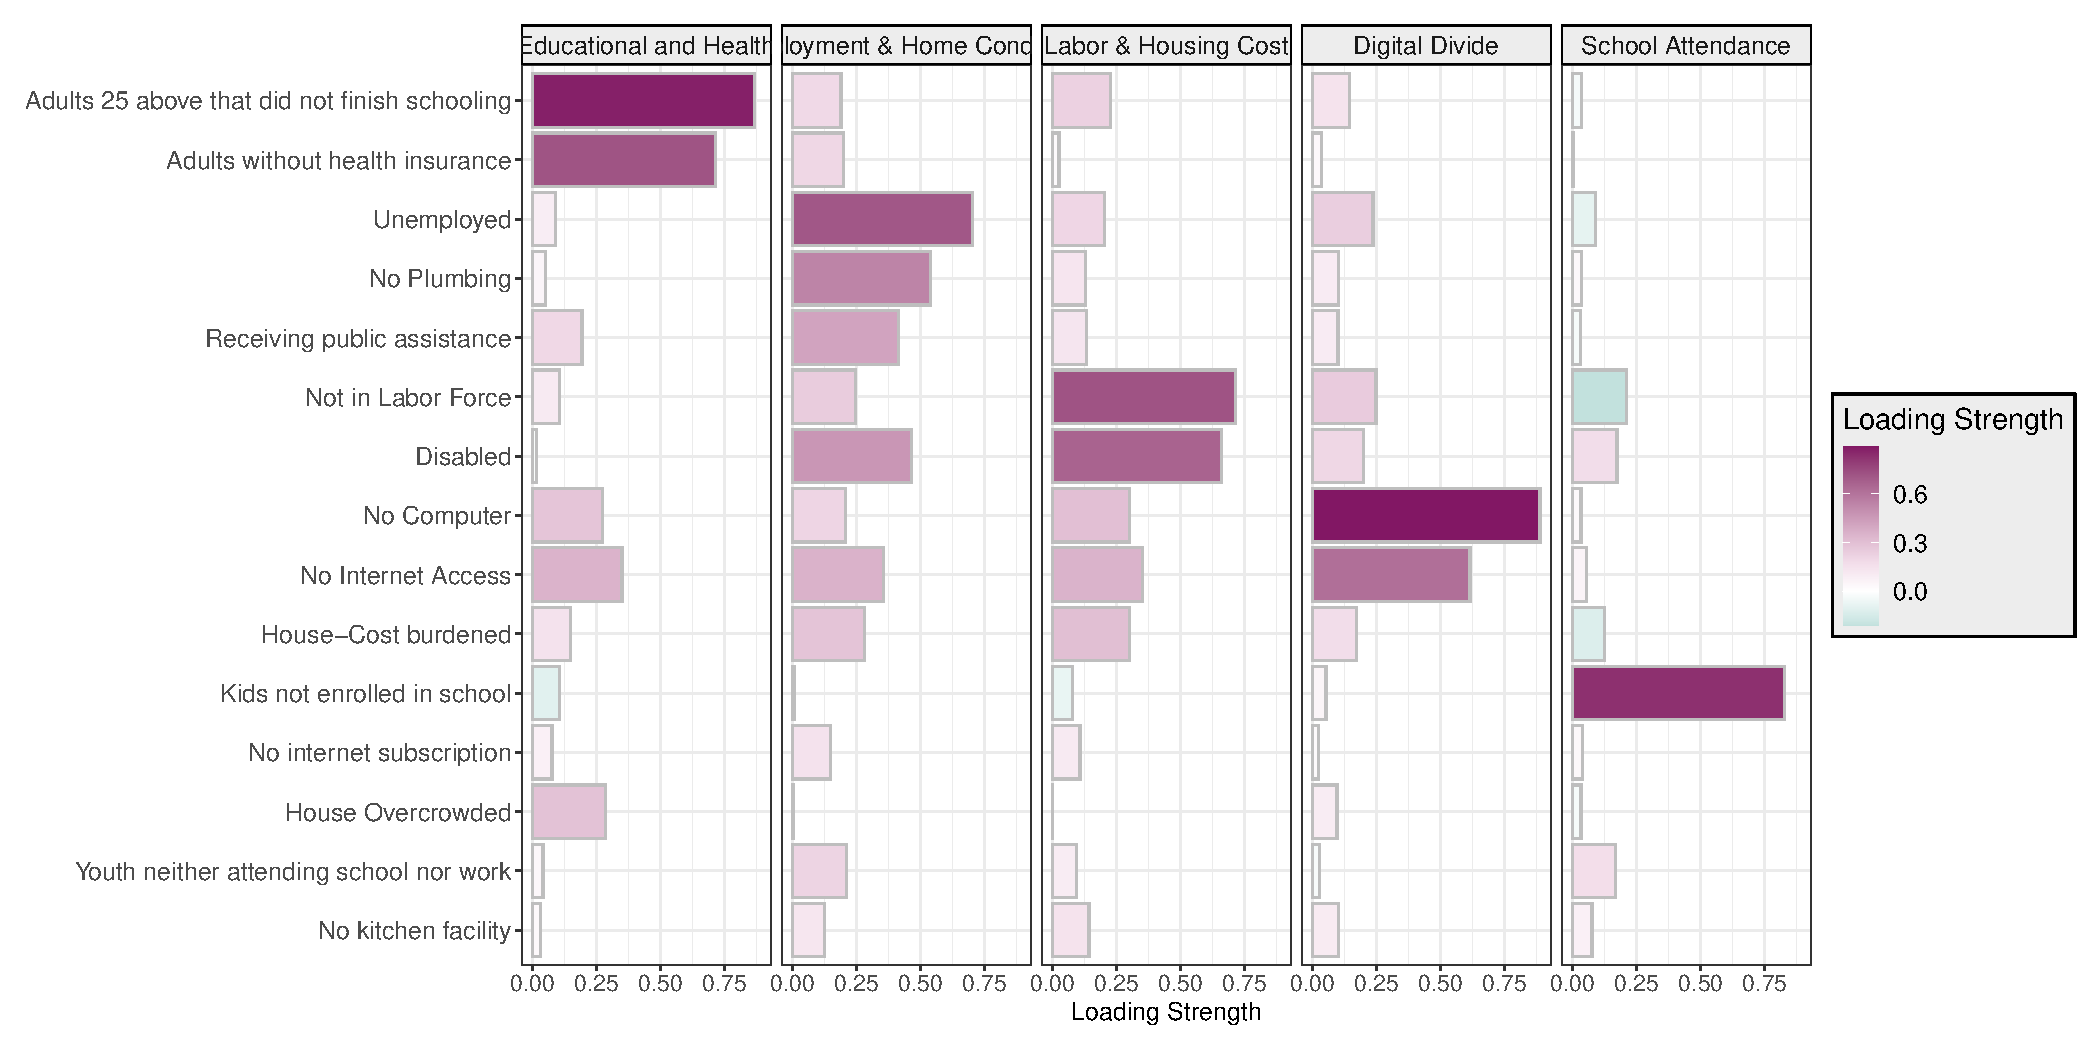
\includegraphics{multidimensional_poverty_files/figure-pdf/viz1-1.pdf}

\bookmarksetup{startatroot}

\chapter{credits}\label{credits}

Developed as a final project for the course MACS 40700 at the University
of Chicago. The author is thankful to Jean Clipperton and Zihua Chen for
the guidance and feedback received throughout the quarter. Special
thanks to Tiwaa Bruks for additional inputs on reading experience.

I benefited from
\href{https://rpubs.com/danmirman/plotting_factor_analysis}{danmirman}
in producing \emph{Figure 1}

Methods for Multidimensional Poverty based on

Alkire, Sabina, and James Foster. ``Counting and multidimensional
poverty measurement.'' Journal of public economics 95, no. 7-8 (2011):
476-487.



\end{document}
